\section{摩擦}\label{sec:3-10}

\begin{wrapfigure}[7]{r}{4cm}
    \centering
    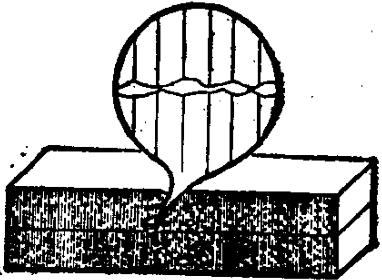
\includegraphics[width=4cm]{../pic/czwl1-ch3-9}
    \caption{}\label{fig:3-9}
\end{wrapfigure}

摩擦是人们经常遇到的现象。我们用手拿起放在桌上的东西,是靠摩擦。假如没有摩擦,手拿东西时它就会滑掉。
我们平常走路,也是靠摩擦。假如没有摩擦,真是寸步难行。你如果在光滑的冰面上滑倒过,就能够体会到这一点。
一般运动物体能够停下来,又是靠摩擦。假如没有摩擦,火车到了站也停不下来,乘客就不能下车。
总之,我们经常遇到并且随时利用摩擦,只是不大注意罢了。现在我们用学过的物理知识来研究这个又有趣又重要的摩擦现象。

一个物体在另一个物体表面上滑动时产生的摩擦,叫做\textbf{滑动摩擦}。
黑板擦跟黑板的摩擦,犁面跟泥土的摩擦,轴跟轴瓦的摩擦,都是滑动摩擦的例子。

产生滑动摩的原因比较复杂,现在还没有完全研究清楚,在这里,我们只能作个粗浅的解释:
看起来十分光滑,互相密合的两个平面,如果放在显微镜下来观察,却象图 \ref{fig:3-9} 那样显示出凹凸不平。
两个物体的凹凸部分互相啮合,当一个物体在另一个物体表面上滑动时,互相啮合的凹凸部分,
就会相互撞碰并且被破坏,阻碍物体运动,这就产生了滑动摩擦。

在滑动摩擦中阻碍物体运动的力,叫做\textbf{摩擦力}。滑动的时侯,摩擦力的方向跟物体运动的方向相反。
摩擦力的大小,可以用图 \ref{fig:3-10} 所示的实验来测量。通过弹簧秤拉着木块在水平桌面上做匀速直线运动。
在水平方向上,木块受到两个力的作用,一个是拉力 $F$,一个是木块和桌面之间的摩擦力 $f$,这两个力的方向相反。
根据上一节讲的可以知道,木块在做匀速运动的时候,它所受的拉力一定等于摩擦力。
从弹簧秤上读出了拉力,也就知道了木块跟桌面之间的摩擦力。

\begin{figure}[htbp]
    \centering
    \begin{minipage}{7cm}
    \centering
    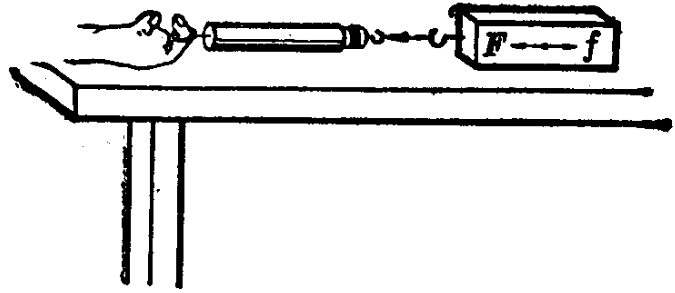
\includegraphics[width=7cm]{../pic/czwl1-ch3-10}
    \caption{}\label{fig:3-10}
    \end{minipage}
    \qquad
    \begin{minipage}{7cm}
    \centering
    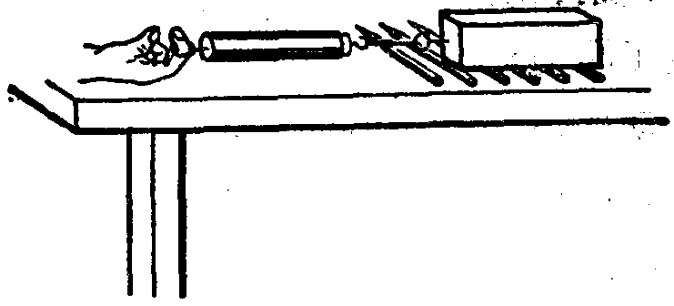
\includegraphics[width=7cm]{../pic/czwl1-ch3-11}
    \caption{}\label{fig:3-11}
    \end{minipage}
\end{figure}


一个物体在另一个物体上滚动时产生的摩擦,叫做\textbf{滚动摩擦}。
汽车、自行车的轮子在地面上滚动时,圆桶或圆木在地面上滚动时,都产生滚动摩擦。

在图 \ref{fig:3-10} 的实验中,如果在木块下面放几支圆铅笔,使滑动摩擦变为滚动摩擦(图 \ref{fig:3-11}),那么弹簧秤的拉力就减小很多。
这说明,滚动摩擦比滑动摩擦小得多。在笨重的设备下面装上小轮,在重物下面垫上几根滚棒,移动起来比较省力,就是因为滚动摩擦小的缘故。


